%%%%%%%%%%%%%%%%%%%%% chapter.tex %%%%%%%%%%%%%%%%%%%%%%%%%%%%%%%%%
%
% sample chapter
%
% Use this file as a template for your own input.
%
%%%%%%%%%%%%%%%%%%%%%%%% Springer-Verlag %%%%%%%%%%%%%%%%%%%%%%%%%%
%\motto{Use the template \emph{chapter.tex} to style the various elements of your chapter content.}

\chapter{Rosetta Code Tasks starting with T}

\section*{Table creation}

In this task, the goal is to create a database table to exemplify most
commonly used data types and options.

See also:

\begin{itemize}
\item
  \emph{Table Creation - Address}
\end{itemize}


\begin{wideverbatim}

(scl 2)

(class +Account +Entity)
(rel id        (+Key +Number))
(rel created   (+Date))
(rel active    (+Bool))
(rel username  (+Key +String))
(rel balance   (+Number) 2)
(rel age       (+Number))
(rel notes     (+Blob))

(pool "account.db")  # Create database

(new! '(+Account)
   'id 12345
   'username "John Doe"
   'balance 77.22
   'created (date 2009 5 13) )

(new! '(+Account)
   'id 12346
   'username "Jane Miller"
   'active T
   'created (date 2009 5 14)
   'balance 123.75 )

(let Fmt (-13 -10 -9 -11 10)
   (tab Fmt "account_id" "created" "active" "username" "balance")
   (for This (collect 'id '+Account)
      (tab Fmt
         (: id)
         (dat\$ (: created))
         (if (: active) "Yes" "No")
         (: username)
         (money (: balance)) ) ) )

Output:

account_id   created   active   username      balance
12345        20090513  No       John Doe        77.22
12346        20090514  Yes      Jane Miller    123.75

\end{wideverbatim}

\pagebreak{}
\section*{Table creation/Postal addresses}

In this task, the goal is to create a table to store addresses. You may
assume that all the addresses to be stored will be located in the USA.
As such, you will need (in addition to a field holding a unique
identifier) a field holding the street address, a field holding the
city, a field holding the state code, and a field holding the zipcode.
Choose appropriate types for each field.

For non-database languages, show how you would open a connection to a
database (your choice of which) and create an address table in it. You
should follow the existing models here for how you would structure the
table.


\begin{wideverbatim}

PicoLisp has built-in database functionality, in the form of (non-relational)
entity/relations built on top of persistent objects (so-called external symbols)

Define an "address" entity, and create the database:

(class +Adr +Entity)
(rel nm (+Sn +Idx +String))            # Name [Soundex index]
(rel str (+String))                    # Street
(rel zip (+Ref +String))               # ZIP [Non-unique index]
(rel cit (+Fold +Idx +String))         # City [Folded substring index]
(rel st (+String))                     # State
(rel tel (+Fold +Ref +String))         # Phone [Folded non-unique index]
(rel em (+Ref +String))                # EMail [Non-unique index]
(rel txt (+Blob))                      # Memo
(rel jpg (+Blob))                      # Photo

(pool "address.db")  # Create database

Create a first entry, and show it:

(show
   (new! '(+Adr)  # Create a record
      'nm "FSF Inc."
      'str "51 Franklin St"
      'st "Boston, MA"
      'zip "02110-1301" ) )

Output:

{2} (+Adr)
   zip "02110-1301"
   st "Boston, MA"
   str "51 Franklin St"
   nm "FSF Inc."

Interactive "select":

(select nm zip +Adr nm "FSF")  # Select name, zip from Adr where name = FSF*
Output:
"FSF Inc." "02110-1301" {2}

\end{wideverbatim}

\pagebreak{}
\section*{Take notes on the command line}


\textbf{Take notes on the command line} is part of \emph{Short
  Circuit}'s \textbf{\emph{Console Program Basics}} selection.

Invoking NOTES without commandline arguments displays the current
contents of the local NOTES.TXT if it exists. If NOTES has arguments,
the current date and time are appended to the local NOTES.TXT followed
by a newline. Then all the arguments, joined with spaces, prepended with
a tab, and appended with a trailing newline, are written to NOTES.TXT.
If NOTES.TXT doesn't already exist in the current directory then a new
NOTES.TXT file should be created.


\begin{wideverbatim}

#!/usr/bin/picolisp /usr/lib/picolisp/lib.l

(load "@lib/misc.l")
(if (argv)
   (out "+notes.txt" (prinl (stamp) "^J^I" (glue " " @)))
   (and (info "notes.txt") (in "notes.txt" (echo))) )
(bye)

\end{wideverbatim}

\pagebreak{}
\section*{Terminal Control/Dimensions}

[aka 'Determine the height and width of the
terminal window']

Determine the height and width of the terminal, and store this
information into variables for subsequent use.

\begin{wideverbatim}

(setq
   Width (in '(tput cols) (read))
   Height (in '(tput lines) (read)) )

\end{wideverbatim}

\pagebreak{}
\section*{Terminal control/Coloured text}

The task is to display a word in various colours on the terminal. The
system palette, or colours such as Red, Green, Blue, Magenta, Cyan, and
Yellow can be used.

Optionally demonstrate:

\begin{itemize}
\item
  How the system should determine if the terminal supports colour
\item
  Setting of the background colour
\item
  How to cause blinking or flashing (if supported by the terminal)
\end{itemize}


\begin{wideverbatim}

(unless (member (sys "TERM") '("linux" "xterm" "rxvt"))
   (quit "This application requires a colour terminal") )

# Coloured text
(for X '((1 . "Red") (4 . "Blue") (3 . "Yellow"))
   (call 'tput "setaf" (car X))
   (prinl (cdr X)) )

# Blinking
(out '(tput "-S")
   (prinl "setab 1^Jsetaf 3^Jblink") )
(prin "Flashing text")

(call 'tput 'sgr0)   # reset
(prinl)

\end{wideverbatim}

\pagebreak{}
\section*{Terminal control/Cursor movement}

The task is to demonstrate how to achieve movement of the terminal
cursor:

\begin{itemize}
\item
  Demonstrate how to move the cursor one position to the left
\item
  Demonstrate how to move the cursor one position to the right
\item
  Demonstrate how to move the cursor up one line (without affecting its
  horizontal position)
\item
  Demonstrate how to move the cursor down one line (without affecting
  its horizontal position)
\item
  Demonstrate how to move the cursor to the beginning of the line
\item
  Demonstrate how to move the cursor to the end of the line
\item
  Demonstrate how to move the cursor to the top left corner of the
  screen
\item
  Demonstrate how to move the cursor to the bottom right corner of the
  screen
\end{itemize}

For the purpose of this task, it is not permitted to overwrite any
characters or attributes on any part of the screen (so outputting a
space is not a suitable solution to achieve a movement to the right).


\begin{wideverbatim}

(call 'tput "cub1")                                # one position to the left
(call 'tput "cuf1")                                # one position to the right
(call 'tput "cuu1")                                # up one line
(call 'tput "cud1")                                # down one line
(call 'tput "cr")                                  # beginning of the line
(call 'tput "hpa" (sys "COLUMNS"))                 # end of the line
(call 'tput "home")                                # top left corner
(call 'tput "cup" (sys "LINES") (sys "COLUMNS"))   # bottom right corner

\end{wideverbatim}

\pagebreak{}
\section*{Terminal control/Preserve screen}

The task is to clear the screen, output something on the display, and
then restore the screen to the preserved state that it was in before the
task was carried out. There is no requirement to change the font or
kerning in this task, however character decorations and attributes are
expected to be preserved. If the implementer decides to change the font
or kerning during the display of the temporary screen, then these
settings need to be restored prior to exit.

\begin{wideverbatim}

#!/usr/bin/picolisp /usr/lib/picolisp/lib.l

(call 'tput "smcup")
(prinl "something")
(wait 3000)
(call 'tput "rmcup")

(bye)

\end{wideverbatim}

\pagebreak{}
\section*{Terminal Control/Unicode output}

The task is to check that the terminal supports Unicode output, before
outputting a Unicode character. If the terminal supports Unicode, then
the terminal should output a Unicode delta (U+25b3). If the terminal
does not support Unicode, then an appropriate error should be raised.

\begin{wideverbatim}

(if (sub? "UTF-8" (or (sys "LC_ALL") (sys "LC_CTYPE") (sys "LANG")))
   (prinl (char (hex "25b3")))
   (quit "UTF-8 capable terminal required") )

\end{wideverbatim}

\pagebreak{}
\section*{Ternary logic}

In \href{http://en.wikipedia.org/wiki/logic}{logic}, a
\textbf{three-valued logic} (also \textbf{trivalent}, \textbf{ternary},
or \textbf{trinary logic}, sometimes abbreviated \textbf{3VL}) is any of
several
\href{http://en.wikipedia.org/wiki/many-valued\_logic}{many-valued
logic} systems in which there are three
\href{http://en.wikipedia.org/wiki/truth\_value}{truth values}
indicating \emph{true}, \emph{false} and some indeterminate third value.
This is contrasted with the more commonly known
\href{http://en.wikipedia.org/wiki/Principle\_of\_bivalence}{bivalent}
logics (such as classical sentential or
\href{http://en.wikipedia.org/wiki/boolean\_logic}{boolean logic}) which
provide only for \emph{true} and \emph{false}. Conceptual form and basic
ideas were initially created by
\href{http://en.wikipedia.org/wiki/Jan\_\%C5\%81ukasiewicz}{Łukasiewicz},
\href{http://en.wikipedia.org/wiki/C.\_I.\_Lewis}{Lewis} and
\href{http://en.wikipedia.org/wiki/Sulski}{Sulski}. These were then
re-formulated by
\href{http://en.wikipedia.org/wiki/Grigore\_Moisil}{Grigore Moisil} in
an axiomatic algebraic form, and also extended to \emph{n}-valued logics
in 1945.

\textbf{Example \emph{Ternary Logic Operators} in \emph{Truth Tables}:}

\ctable[caption = {\emph{not} a }, pos = H, center, botcap]{ll}
{% notes
}
{% rows
\FL
¬
\ML
True & False
\\\noalign{\medskip}
Maybe & Maybe
\\\noalign{\medskip}
False & True
\LL
}

a \emph{and} b

∧

True

Maybe

False

True

True

Maybe

False

Maybe

Maybe

Maybe

False

False

False

False

False

a \emph{or} b

∨

True

Maybe

False

True

True

True

True

Maybe

True

Maybe

Maybe

False

True

Maybe

False

\emph{if} a \emph{then} b

⊃

True

Maybe

False

True

True

Maybe

False

Maybe

True

Maybe

Maybe

False

True

True

True

a \emph{is equivalent to} b

≡

True

Maybe

False

True

True

Maybe

False

Maybe

Maybe

Maybe

Maybe

False

False

Maybe

True

\textbf{Task:}

\begin{itemize}
\item
  Define a new type that emulates \emph{ternary logic} by storing data
  \textbf{trits}.
\item
  Given all the binary logic operators of the original programming
  language, reimplement these operators for the new \emph{Ternary logic}
  type \textbf{trit}.
\item
  Generate a sampling of results using \textbf{trit} variables.
\item
  \href{http://en.wikipedia.org/wiki/Kudos}{Kudos} for actually thinking
  up a test case algorithm where \emph{ternary logic} is intrinsically
  useful, optimises the test case algorithm and is preferable to binary
  logic.
\end{itemize}

Note: \textbf{\href{http://en.wikipedia.org/wiki/Setun}{Setun}} (Сетунь)
was a \href{http://en.wikipedia.org/wiki/balanced\_ternary}{balanced
ternary} computer developed in 1958 at
\href{http://en.wikipedia.org/wiki/Moscow\_State\_University}{Moscow
State University}. The device was built under the lead of
\href{http://en.wikipedia.org/wiki/Sergei\_Sobolev}{Sergei Sobolev} and
\href{http://en.wikipedia.org/wiki/Nikolay\_Brusentsov}{Nikolay
Brusentsov}. It was the only modern
\href{http://en.wikipedia.org/wiki/ternary\_computer}{ternary computer},
using three-valued
\href{http://en.wikipedia.org/wiki/ternary\_logic}{ternary logic}



\begin{wideverbatim}

In addition for the standard T (for "true") and NIL (for "false") we define 0
(zero, for "maybe").

(de 3not (A)
   (or (=0 A) (not A)) )

(de 3and (A B)
   (cond
      ((=T A) B)
      ((=0 A) (and B 0)) ) )

(de 3or (A B)
   (cond
      ((=T A) T)
      ((=0 A) (or (=T B) 0))
      (T B) ) )

(de 3impl (A B)
   (cond
      ((=T A) B)
      ((=0 A) (or (=T B) 0))
      (T T) ) )

(de 3equiv (A B)
   (cond
      ((=T A) B)
      ((=0 A) 0)
      (T (3not B)) ) )

Test:

(for X '(T 0 NIL)
   (println 'not X '-> (3not X)) )

(for Fun '((and . 3and) (or . 3or) (implies . 3impl) (equivalent . 3equiv))
   (for X '(T 0 NIL)
      (for Y '(T 0 NIL)
         (println X (car Fun) Y '-> ((cdr Fun) X Y)) ) ) )


\end{wideverbatim}

\begin{wideverbatim}

Output:

not T -> NIL
not 0 -> 0
not NIL -> T
T and T -> T
T and 0 -> 0
T and NIL -> NIL
0 and T -> 0
0 and 0 -> 0
0 and NIL -> NIL
NIL and T -> NIL
NIL and 0 -> NIL
NIL and NIL -> NIL
T or T -> T
T or 0 -> T
T or NIL -> T
0 or T -> T
0 or 0 -> 0
0 or NIL -> 0
NIL or T -> T
NIL or 0 -> 0
NIL or NIL -> NIL
T implies T -> T
T implies 0 -> 0
T implies NIL -> NIL
0 implies T -> T
0 implies 0 -> 0
0 implies NIL -> 0
NIL implies T -> T
NIL implies 0 -> T
NIL implies NIL -> T
T equivalent T -> T
T equivalent 0 -> 0
T equivalent NIL -> NIL
0 equivalent T -> 0
0 equivalent 0 -> 0
0 equivalent NIL -> 0
NIL equivalent T -> NIL
NIL equivalent 0 -> 0
NIL equivalent NIL -> T

\end{wideverbatim}

\pagebreak{}
\section*{Test a function}

Using a well known testing specific library/module/suite for your
language, write some tests for your language's entry in
\emph{Palindrome}. If your language does not have a
testing specific library well known to the language's community then
state this or omit the language.


\begin{wideverbatim}

The '[http://software-lab.de/doc/refT.html#test test]' function is
built into PicoLisp.

(de palindrome? (S)
   (= (setq S (chop S)) (reverse S)) )

(test T (palindrome? "racecar"))
(test NIL (palindrome? "ferrari"))

\end{wideverbatim}

\pagebreak{}
\section*{Text processing/1}

Often data is produced by one program, in the wrong format for later
use by another program or person. In these situations another program
can be written to parse and transform the original data into a format
useful to the other. The term ``Data Munging'' is
\href{http://www.google.co.uk/search?q=\%22data+munging\%22}{often}
used in programming circles for this task.

A
\href{http://groups.google.co.uk/group/comp.lang.awk/msg/0ecba3a3fbf247d8?hl=en}{request}
on the comp.lang.awk newsgroup lead to a typical data munging task:

\begin{wideverbatim}
I have to analyse data files that have the following format:
Each row corresponds to 1 day and the field logic is: $1 is the date,
followed by 24 value/flag pairs, representing measurements at 01:00,
02:00 ... 24:00 of the respective day. In short:

<date> <val1> <flag1> <val2> <flag2> ...  <val24> <flag24>

Some test data is available at: 
... (nolonger available at original location)

I have to sum up the values (per day and only valid data, i.e. with
flag>0) in order to calculate the mean. That's not too difficult.
However, I also need to know what the "maximum data gap" is, i.e. the
longest period with successive invalid measurements (i.e values with
flag<=0)
\end{wideverbatim}

The data is
\href{http://www.eea.europa.eu/help/eea-help-centre/faqs/how-do-i-obtain-eea-reports}{free
to download and use} and is of this format:

\begin{wideverbatim}
1991-03-30  10.000  1   10.000  1   10.000  1   10.000  1   10.000  1   10.000  1   10.000  1   10.000  1   10.000  1   10.000  1   10.000  1   10.000  1   10.000  1   10.000  1   10.000  1   10.000  1   10.000  1   10.000  1   10.000  1   10.000  1   10.000  1   10.000  1   10.000  1   10.000  1
1991-03-31  10.000  1   10.000  1   10.000  1   10.000  1   10.000  1   10.000  1   10.000  1   20.000  1   20.000  1   20.000  1   35.000  1   50.000  1   60.000  1   40.000  1   30.000  1   30.000  1   30.000  1   25.000  1   20.000  1   20.000  1   20.000  1   20.000  1   20.000  1   35.000  1
1991-03-31  40.000  1   0.000   -2  0.000   -2  0.000   -2  0.000   -2  0.000   -2  0.000   -2  0.000   -2  0.000   -2  0.000   -2  0.000   -2  0.000   -2  0.000   -2  0.000   -2  0.000   -2  0.000   -2  0.000   -2  0.000   -2  0.000   -2  0.000   -2  0.000   -2  0.000   -2  0.000   -2  0.000   -2
1991-04-01  0.000   -2  13.000  1   16.000  1   21.000  1   24.000  1   22.000  1   20.000  1   18.000  1   29.000  1   44.000  1   50.000  1   43.000  1   38.000  1   27.000  1   27.000  1   24.000  1   23.000  1   18.000  1   12.000  1   13.000  1   14.000  1   15.000  1   13.000  1   10.000  1
1991-04-02  8.000   1   9.000   1   11.000  1   12.000  1   12.000  1   12.000  1   27.000  1   26.000  1   27.000  1   33.000  1   32.000  1   31.000  1   29.000  1   31.000  1   25.000  1   25.000  1   24.000  1   21.000  1   17.000  1   14.000  1   15.000  1   12.000  1   12.000  1   10.000  1
1991-04-03  10.000  1   9.000   1   10.000  1   10.000  1   9.000   1   10.000  1   15.000  1   24.000  1   28.000  1   24.000  1   18.000  1   14.000  1   12.000  1   13.000  1   14.000  1   15.000  1   14.000  1   15.000  1   13.000  1   13.000  1   13.000  1   12.000  1   10.000  1   10.000  1
\end{wideverbatim}

Only a sample of the data showing its format is given above. The full
example file may be downloaded
\href{http://rosettacode.org/resources/readings.zip}{here}.

Structure your program to show statistics for each line of the file,
(similar to the original Python, Perl, and AWK examples below), followed
by summary statistics for the file. When showing example output just
show a few line statistics and the full end summary.



\begin{wideverbatim}



Put the following into an executable file "readings":

#!/usr/bin/picolisp /usr/lib/picolisp/lib.l

(let (NoData 0  NoDataMax -1  NoDataMaxline "!"  TotFile 0  NumFile 0)
   (let InFiles
      (glue ","
         (mapcar
            '((File)
               (in File
                  (while (split (line) "^I")
                     (let (Len (length @)  Date (car @)  TotLine 0  NumLine 0)
                        (for (L (cdr @)  L  (cddr L))
                           (if (> 1 (format (cadr L)))
                              (inc 'NoData)
                              (when (gt0 NoData)
                                 (when (= NoDataMax NoData)
                                    (setq NoDataMaxline (pack NoDataMaxline ", " Date)) )
                                 (when (> NoData NoDataMax)
                                    (setq NoDataMax NoData  NoDataMaxline Date) ) )
                              (zero NoData)
                              (inc 'TotLine (format (car L) 3))
                              (inc 'NumLine) ) )
                        (inc 'TotFile TotLine)
                        (inc 'NumFile NumLine)
                        (tab (-7 -12 -7 3 -9 3 -11 11 -11 11)
                           "Line:" Date
                           "Reject:" (- (/ (dec Len) 2) NumLine)
                           "  Accept:" NumLine
                           "  Line_tot:" (format TotLine 3)
                           "  Line_avg:"
                           (and (gt0 NumLine) (format (*/ TotLine @) 3)) ) ) ) )
               File )
            (argv) ) )
      (prinl)
      (prinl "File(s)  = " InFiles)
      (prinl "Total    = " (format TotFile 3))
      (prinl "Readings = " NumFile)
      (prinl "Average  = " (format (*/ TotFile NumFile) 3))
      (prinl)
      (prinl
         "Maximum run(s) of " NoDataMax
         " consecutive false readings ends at line starting with
         date(s): " NoDataMaxline ) ) )

(bye)

\end{wideverbatim}

\begin{wideverbatim}


Then it can be called as

\$ ./readings readings.txt |tail
Line:  2004-12-29  Reject: 1 Accept: 23  Line_tot: 56.300  Line_avg: 2.448
Line:  2004-12-30  Reject: 1 Accept: 23  Line_tot: 65.300  Line_avg: 2.839
Line:  2004-12-31  Reject: 1 Accept: 23  Line_tot: 47.300  Line_avg: 2.057

File(s)  = readings.txt
Total    = 1358393.400
Readings = 129403
Average  = 10.497

Maximum run(s) of 589 consecutive false readings ends at line starting
with date(s): 1993-03-05
\$

\end{wideverbatim}

\pagebreak{}
\section*{Text processing/2}

The following data shows a few lines from the file readings.txt (as used
in the \emph{Data Munging} task).

The data comes from a pollution monitoring station with twenty four
instruments monitoring twenty four aspects of pollution in the air.
Periodically a record is added to the file constituting a line of 49
white-space separated fields, where white-space can be one or more space
or tab characters.

The fields (from the left) are:

\begin{verbatim}
 DATESTAMP [ VALUEn FLAGn ] * 24
\end{verbatim}

i.e. a datestamp followed by twenty four repetitions of a floating point
instrument value and that instruments associated integer flag. Flag
values are \textgreater{}= 1 if the instrument is working and
\textless{} 1 if there is some problem with that instrument, in which
case that instrument's value should be ignored.

A sample from the full data file
\href{http://rosettacode.org/resources/readings.zip}{readings.txt} is:

\begin{wideverbatim}
1991-03-30  10.000  1   10.000  1   10.000  1   10.000  1   10.000  1   10.000  1   10.000  1   10.000  1   10.000  1   10.000  1   10.000  1   10.000  1   10.000  1   10.000  1   10.000  1   10.000  1   10.000  1   10.000  1   10.000  1   10.000  1   10.000  1   10.000  1   10.000  1   10.000  1
1991-03-31  10.000  1   10.000  1   10.000  1   10.000  1   10.000  1   10.000  1   10.000  1   20.000  1   20.000  1   20.000  1   35.000  1   50.000  1   60.000  1   40.000  1   30.000  1   30.000  1   30.000  1   25.000  1   20.000  1   20.000  1   20.000  1   20.000  1   20.000  1   35.000  1
1991-03-31  40.000  1   0.000   -2  0.000   -2  0.000   -2  0.000   -2  0.000   -2  0.000   -2  0.000   -2  0.000   -2  0.000   -2  0.000   -2  0.000   -2  0.000   -2  0.000   -2  0.000   -2  0.000   -2  0.000   -2  0.000   -2  0.000   -2  0.000   -2  0.000   -2  0.000   -2  0.000   -2  0.000   -2
1991-04-01  0.000   -2  13.000  1   16.000  1   21.000  1   24.000  1   22.000  1   20.000  1   18.000  1   29.000  1   44.000  1   50.000  1   43.000  1   38.000  1   27.000  1   27.000  1   24.000  1   23.000  1   18.000  1   12.000  1   13.000  1   14.000  1   15.000  1   13.000  1   10.000  1
1991-04-02  8.000   1   9.000   1   11.000  1   12.000  1   12.000  1   12.000  1   27.000  1   26.000  1   27.000  1   33.000  1   32.000  1   31.000  1   29.000  1   31.000  1   25.000  1   25.000  1   24.000  1   21.000  1   17.000  1   14.000  1   15.000  1   12.000  1   12.000  1   10.000  1
1991-04-03  10.000  1   9.000   1   10.000  1   10.000  1   9.000   1   10.000  1   15.000  1   24.000  1   28.000  1   24.000  1   18.000  1   14.000  1   12.000  1   13.000  1   14.000  1   15.000  1   14.000  1   15.000  1   13.000  1   13.000  1   13.000  1   12.000  1   10.000  1   10.000  1
\end{wideverbatim}

The task:

\begin{enumerate}
\item
  Confirm the general field format of the file
\item
  Identify any DATESTAMPs that are duplicated.
\item
  What number of records have good readings for all instruments.
\end{enumerate}



\begin{wideverbatim}

Put the following into an executable file "checkReadings":

#!/usr/bin/picolisp /usr/lib/picolisp/lib.l

(load "@lib/misc.l")

(in (opt)
   (until (eof)
      (let Lst (split (line) "^I")
         (unless
            (and
               (= 49 (length Lst))     # Check total length
               (\$dat (car Lst) "-")    # Check for valid date
               (not
                  (find                # Check data format
                     '((L F)
                        (not
                           (if F                            # Alternating:
                              (format L 3)                  # Number
                              (>= 9 (format L) -9) ) ) )    # or flag
                     (cdr Lst)
                     '(T NIL .) ) ) )
            (prinl "Bad line format: " (glue " " Lst))
            (bye 1) ) ) ) )

(bye)

Then it can be called as

\$ ./checkReadings readings.txt

\end{wideverbatim}

\pagebreak{}
\section*{Text processing/3}
[aka 'Text processing/Max licenses in use']

A company currently pays a fixed sum for the use of a particular
licensed software package. In determining if it has a good deal it
decides to calculate its maximum use of the software from its license
management log file.

Assume the software's licensing daemon faithfully records a checkout
event when a copy of the software starts and a checkin event when the
software finishes to its log file. An example of checkout and checkin
events are:

\begin{verbatim}
 License OUT @ 2008/10/03_23:51:05 for job 4974
 ...
 License IN  @ 2008/10/04_00:18:22 for job 4974
\end{verbatim}

Save the 10,000 line log file from
\href{http://rosettacode.org/resources/mlijobs.txt}{here} into a local
file then write a program to scan the file extracting both the maximum
licenses that were out at any time, and the time(s) at which this
occurs.


\begin{wideverbatim}

Put the following into an executable file "licenses":

#!/usr/bin/picolisp /usr/lib/picolisp/lib.l

(zero Count MaxCount)

(in (opt)
   (while (split (line) " ")
      (case (pack (cadr (setq Line @)))
         (IN
            (dec 'Count) )
         (OUT
            (let Time (cadddr Line)
               (cond
                  ((> (inc 'Count) MaxCount)
                     (setq MaxCount Count  MaxTimes Time) )
                  ((= Count MaxCount)
                     (setq MaxTimes (pack MaxTimes " and " Time)) ) ) ) ) ) ) )

(prinl "The biggest number of licenses is " MaxCount " at " MaxTimes " !")
(bye)

Then it can be called as

\$ ./licenses mlijobs.txt
The biggest number of licenses is 99 at 2008/10/03_08:39:34 and 2008/10/03_08:40:40 !

\end{wideverbatim}

\pagebreak{}
\section*{Thiele's interpolation formula}

\textbf{\href{http://en.wikipedia.org/wiki/Thiele\%27s\_interpolation\_formula}{Thiele's
interpolation formula}} is an interpolation formula for a function
\emph{f}(•) of a single variable. It is expressed as a
\emph{continued fraction}:

\begin{figure}[H]
\centering
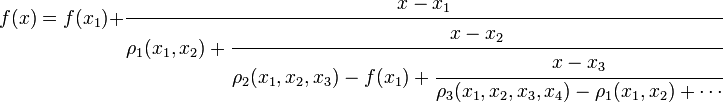
\includegraphics[scale=.6]{graphics/64932f8d89d7f1750d3d40723007bd27.png}
% \caption{ f(x) = f(x\_1) +
% \textbackslash{}cfrac\{x-x\_1\}\{\textbackslash{}rho\_1(x\_1,x\_2) +
% \textbackslash{}cfrac\{x-x\_2\}\{\textbackslash{}rho\_2(x\_1,x\_2,x\_3)
% - f(x\_1) +
% \textbackslash{}cfrac\{x-x\_3\}\{\textbackslash{}rho\_3(x\_1,x\_2,x\_3,x\_4)
% - \textbackslash{}rho\_1(x\_1,x\_2) + \textbackslash{}cdots\}\}\} }
\end{figure}

ρ represents the
\href{http://en.wikipedia.org/wiki/reciprocal\_difference}{reciprocal
difference}, demonstrated here for reference:

\begin{figure}[H]
\centering
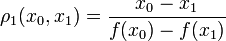
\includegraphics[scale=.6]{graphics/f7e030787df8cd5d0ed6dd1802306d11.png}
% \caption{\textbackslash{}rho\_1(x\_0, x\_1) = \textbackslash{}frac\{x\_0
% - x\_1\}\{f(x\_0) - f(x\_1)\}}
\end{figure}

\begin{figure}[H]
\centering
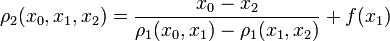
\includegraphics[scale=.6]{graphics/447c2e5168e15cb21cafda55903db017.png}
% \caption{\textbackslash{}rho\_2(x\_0, x\_1, x\_2) =
% \textbackslash{}frac\{x\_0 - x\_2\}\{\textbackslash{}rho\_1(x\_0, x\_1)
% - \textbackslash{}rho\_1(x\_1, x\_2)\} + f(x\_1)}
\end{figure}

\begin{figure}[H]
\centering
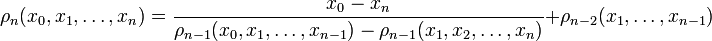
\includegraphics[scale=.6]{graphics/c7be4230ba817ec495c68f3c5fa10cfb.png}
% \caption{\textbackslash{}rho\_n(x\_0,x\_1,\textbackslash{}ldots,x\_n)=\textbackslash{}frac\{x\_0-x\_n\}\{\textbackslash{}rho\_\{n-1\}(x\_0,x\_1,\textbackslash{}ldots,x\_\{n-1\})-\textbackslash{}rho\_\{n-1\}(x\_1,x\_2,\textbackslash{}ldots,x\_n)\}+\textbackslash{}rho\_\{n-2\}(x\_1,\textbackslash{}ldots,x\_\{n-1\})}
\end{figure}

Demonstrate Thiele's interpolation function by:

\begin{enumerate}
\item
  Building a 32 row \emph{trig table} of values of the trig functions
  \emph{sin}, \emph{cos} and \emph{tan}. e.g. \textbf{for} x
  \textbf{from} 0 \textbf{by} 0.05 \textbf{to} 1.55\ldots{}
\item
  Using columns from this table define an inverse - using Thiele's
  interpolation - for each trig function;
\item
  Finally: demonstrate the following well known trigonometric
  identities:

  \begin{itemize}
  \item
    6 × sin\textsuperscript{-1} ½ = π
  \item
    3 × cos\textsuperscript{-1} ½ = π
  \item
    4 × tan\textsuperscript{-1} 1 = π
  \end{itemize}
\end{enumerate}

\begin{wideverbatim}

(scl 17)
(load "@lib/math.l")

(setq
   *X-Table (range 0.0 1.55 0.05)
   *SinTable (mapcar sin *X-Table)
   *CosTable (mapcar cos *X-Table)
   *TanTable (mapcar tan *X-Table)
   *TrigRows (length *X-Table) )

(let N2 (>> 1 (* *TrigRows (dec *TrigRows)))
   (setq
      *InvSinTable (need N2)
      *InvCosTable (need N2)
      *InvTanTable (need N2) ) )

(de rho (Tbl Inv I N)
   (cond
      ((lt0 N) 0)
      ((=0 N) (get *X-Table I))
      (T
         (let Idx (+ I (>> 1 (* (- *TrigRows 1 N) (- *TrigRows N))))
            (or
               (get Inv Idx)
               (set (nth Inv Idx)  # only happens if value not computed yet
                  (+
                     (rho Tbl Inv (inc I) (- N 2))
                     (*/
                        (- (get Tbl I) (get Tbl (+ I N)))
                        1.0
                        (-
                           (rho Tbl Inv I (dec N))
                           (rho Tbl Inv (inc I) (dec N)) ) ) ) ) ) ) ) ) )

(de thiele (Tbl Inv X N)
   (if (> N *TrigRows)
      1.0
      (+
         (-
            (rho Tbl Inv 1 (dec N))
            (rho Tbl Inv 1 (- N 3)) )
         (*/
            (- X (get Tbl N))
            1.0
            (thiele Tbl Inv X (inc N)) ) ) ) )

\end{wideverbatim}

\begin{wideverbatim}

(de iSin (X)
   (thiele *SinTable *InvSinTable X 1) )

(de iCos (X)
   (thiele *CosTable *InvCosTable X 1) )

(de iTan (X)
   (thiele *TanTable *InvTanTable 1.0 1) )

Test:

(prinl (round (* 6 (iSin 0.5)) 15))
(prinl (round (* 3 (iCos 0.5)) 15))
(prinl (round (* 4 (iTan 1.0)) 15))

Output:

3.141592653589793
3.141592653589793
3.141592653589793

\end{wideverbatim}

\pagebreak{}
\section*{Three Dogs}
[aka 'Case-sensitivity of identifiers']

Three dogs (Are there three dogs or one dog?) is a code snippet used to
illustrate the lettercase sensitivity of the programming language. For a
case-sensitive language, the identifiers dog, Dog and DOG are all
different and we should get the output:

The three dogs are named Benjamin, Samba and Bernie.

For a language that is lettercase insensitive, we get the following
output:

There is just one dog named Bernie.

\begin{description}
\item[Cf.]
\end{description}

\begin{itemize}
\item \emph{Unicode variable names}
\end{itemize}


\begin{wideverbatim}

(let (dog "Benjamin"  Dog "Samba"  DOG "Bernie")
   (prinl "The three dogs are named " dog ", " Dog " and " DOG) )

Output:

The three dogs are named Benjamin, Samba and Bernie

\end{wideverbatim}

\pagebreak{}
\section*{Tic-tac-toe}

Play a game of
\href{http://en.wikipedia.org/wiki/Tic-tac-toe}{tic-tac-toe}. Ensure
that legal moves are played and that a winning position is notified.

\begin{wideverbatim}

This solution doesn't bother about the game logic, but simply uses
the alpha-beta-pruning 'game' function in the "simul" library.

(load "@lib/simul.l")  # for 'game' function
 
(de display ()
   (for Y (3 2 1)
      (prinl "   +---+---+---+")
      (prin " " Y)
      (for X (1 2 3)
         (prin " | " (or (get *Board X Y) " ")) )
      (prinl " |") )
   (prinl "   +---+---+---+")
   (prinl "     a   b   c") )
 
(de find3 (P)
   (find
      '((X Y DX DY)
         (do 3
            (NIL (= P (get *Board X Y)))
            (inc 'X DX)
            (inc 'Y DY)
            T ) )
      (1 1 1 1 2 3 1 1)
      (1 2 3 1 1 1 1 3)
      (1 1 1 0 0 0 1 1)
      (0 0 0 1 1 1 1 -1) ) )
 
\end{wideverbatim}

\begin{wideverbatim}


(de myMove ()
   (when
      (game NIL 8
         '((Flg)     # Moves
            (unless (find3 (or (not Flg) 0))
               (make
                  (for (X . L) *Board
                     (for (Y . P) L
                        (unless P
                           (link
                              (cons
                                 (cons X Y (or Flg 0))
                                 (list X Y) ) ) ) ) ) ) ) )
         '((Mov) # Move
            (set (nth *Board (car Mov) (cadr Mov)) (cddr Mov)) )
         '((Flg)     # Cost
            (if (find3 (or Flg 0)) -100 0) ) )
      (let Mov (caadr @)
         (set (nth *Board (car Mov) (cadr Mov)) 0) )
      (display) ) )
 
(de yourMove (X Y)
   (and
      (sym? X)
      (>= 3 (setq X (- (char X) 96)) 1)
      (num? Y)
      (>= 3 Y 1)
      (not (get *Board X Y))
      (set (nth *Board X Y) T)
      (display) ) )
 
(de main ()
   (setq *Board (make (do 3 (link (need 3)))))
   (display) )
 
(de go Args
   (cond
      ((not (yourMove (car Args) (cadr Args)))
         "Illegal move!" )
      ((find3 T) "Congratulation, you won!")
      ((not (myMove)) "No moves")
      ((find3 0) "Sorry, you lost!") ) )

\end{wideverbatim}

\begin{wideverbatim}


Output:

: (main)
   +---+---+---+
 3 |   |   |   |
   +---+---+---+
 2 |   |   |   |
   +---+---+---+
 1 |   |   |   |
   +---+---+---+
     a   b   c

: (go a 1)
   +---+---+---+
 3 |   |   |   |
   +---+---+---+
 2 |   |   |   |
   +---+---+---+
 1 | T |   |   |
   +---+---+---+
     a   b   c
   +---+---+---+
 3 |   |   |   |
   +---+---+---+
 2 |   | 0 |   |
   +---+---+---+
 1 | T |   |   |
   +---+---+---+
     a   b   c

\end{wideverbatim}

\pagebreak{}
\section*{Time a function}

Write a program which uses a timer (with the least granularity available
on your system) to time how long a function takes to execute.

Whenever possible, use methods which measure only the processing time
used by the current process; instead of the difference in
\emph{system time} between start and finish, which
could include time used by other processes on the computer.

This task is intended as a subtask for \emph{Measure relative
  performance of sorting algorithms implementations}.


\begin{wideverbatim}

There is a built-in function '[http://software-lab.de/doc/refB.html#bench bench]
for that. However, it measures wall-clock time, because for practical purposes
the real time needed by a task (including I/O and communication) is more meaning
There is another function, '[http://software-lab.de/doc/refT.html#tick tick]', w
also measures user time, and is used by the profiling tools.

: (bench (do 1000000 (* 3 4)))
0.080 sec
-> 12

\end{wideverbatim}

% \pagebreak{}
% \section*{Tokenize a string}

% Separate the string ``Hello,How,Are,You,Today'' by commas into an array
% (or list) so that each element of it stores a different word. Display
% the words to the `user', in the simplest manner possible, separated by a
% period. To simplify, you may display a trailing period.


% \begin{wideverbatim}

% {Arm}

% \end{wideverbatim}

\pagebreak{}
\section*{Top rank per group}

Find the top \emph{N} salaries in each department, where \emph{N} is
provided as a parameter.

Use this data as a formatted internal data structure (adapt it to your
language-native idioms, rather than parse at runtime), or identify your
external data source:

\begin{verbatim}
Employee Name,Employee ID,Salary,Department
Tyler Bennett,E10297,32000,D101
John Rappl,E21437,47000,D050
George Woltman,E00127,53500,D101
Adam Smith,E63535,18000,D202
Claire Buckman,E39876,27800,D202
David McClellan,E04242,41500,D101
Rich Holcomb,E01234,49500,D202
Nathan Adams,E41298,21900,D050
Richard Potter,E43128,15900,D101
David Motsinger,E27002,19250,D202
Tim Sampair,E03033,27000,D101
Kim Arlich,E10001,57000,D190
Timothy Grove,E16398,29900,D190
\end{verbatim}


\begin{wideverbatim}

# Employee Name, ID, Salary, Department
(de *Employees
   ("Tyler Bennett" E10297 32000 D101)
   ("John Rappl" E21437 47000 D050)
   ("George Woltman" E00127 53500 D101)
   ("Adam Smith" E63535 18000 D202)
   ("Claire Buckman" E39876 27800 D202)
   ("David McClellan" E04242 41500 D101)
   ("Rich Holcomb" E01234 49500 D202)
   ("Nathan Adams" E41298 21900 D050)
   ("Richard Potter" E43128 15900 D101)
   ("David Motsinger" E27002 19250 D202)
   ("Tim Sampair" E03033 27000 D101)
   ("Kim Arlich" E10001 57000 D190)
   ("Timothy Grove" E16398 29900 D190) )

(de topEmployees (N)
   (let Fmt (4 -16 -7 7)
      (for Dept (by cadddr group *Employees)
         (prinl "Department " (cadddr (car Dept)) ":")
         (tab Fmt NIL "Name" "ID" "Salary")
         (for (I . D) (flip (by caddr sort Dept))
            (tab Fmt (pack I ". ") (car D) (cadr D) (caddr D))
            (T (= I N)) )
         (prinl) ) ) )

(topEmployees 3)

Output:

Department D101:
    Name            ID      Salary
 1. George Woltman  E00127   53500
 2. David McClellan E04242   41500
 3. Tyler Bennett   E10297   32000

Department D050:
    Name            ID      Salary
 1. John Rappl      E21437   47000
 2. Nathan Adams    E41298   21900

Department D202:
    Name            ID      Salary
 1. Rich Holcomb    E01234   49500
 2. Claire Buckman  E39876   27800
 3. David Motsinger E27002   19250

Department D190:
    Name            ID      Salary
 1. Kim Arlich      E10001   57000
 2. Timothy Grove   E16398   29900

\end{wideverbatim}

\pagebreak{}
\section*{Topological sort}

Given a mapping between items, and items they depend on, a
\href{http://en.wikipedia.org/wiki/Topological\_sorting}{topological
sort} orders items so that no item precedes an item it depends upon.

The compiling of a library in the
\href{http://en.wikipedia.org/wiki/VHDL}{VHDL} language has the
constraint that a library must be compiled after any library it depends
on. A tool exists that extracts library dependencies. The task is to
\textbf{write a function that will return a valid compile order of VHDL
libraries from their dependencies.}

\begin{itemize}
\item
  Assume library names are single words.
\item
  Items mentioned as only dependants, (sic), have no dependants of their
  own, but their order of compiling must be given.
\item
  Any self dependencies should be ignored.
\item
  Any un-orderable dependencies should be flagged.
\end{itemize}

Use the following data as an example:

\begin{wideverbatim}
LIBRARY          LIBRARY DEPENDENCIES
=======          ====================
des_system_lib   std synopsys std_cell_lib des_system_lib dw02 dw01 ramlib ieee
dw01             ieee dw01 dware gtech
dw02             ieee dw02 dware
dw03             std synopsys dware dw03 dw02 dw01 ieee gtech
dw04             dw04 ieee dw01 dware gtech
dw05             dw05 ieee dware
dw06             dw06 ieee dware
dw07             ieee dware
dware            ieee dware
gtech            ieee gtech
ramlib           std ieee
std_cell_lib     ieee std_cell_lib
synopsys         
\end{wideverbatim}

Note: the above data would be un-orderable if, for example,
\texttt{dw04} is added to the list of dependencies of \texttt{dw01}.

C.f: \emph{Topological sort/Extracted top item}.



\begin{wideverbatim}

(de sortDependencies (Lst)
   (setq Lst                              # Build a flat list
      (uniq
         (mapcan
            '((L)
               (put (car L) 'dep (cdr L)) # Store dependencies in 'dep' properties
               (copy L) )
            (mapcar uniq Lst) ) ) )       # without self-dependencies
   (make
      (while Lst
         (ifn (find '((This) (not (: dep))) Lst)   # Found non-depending lib?
            (quit "Can't resolve dependencies" Lst)
            (del (link @) 'Lst)                    # Yes: Store in result
            (for This Lst                          # and remove from 'dep's
               (=: dep (delete @ (: dep))) ) ) ) ) )

Output:

: (sortDependencies
   (quote
      (des-system-lib   std synopsys std-cell-lib des-system-lib dw02 dw01 ramlib ieee)
      (dw01             ieee dw01 dware gtech)
      (dw02             ieee dw02 dware)
      (dw03             std synopsys dware dw03 dw02 dw01 ieee gtech)
      (dw04             dw04 ieee dw01 dware gtech)
      (dw05             dw05 ieee dware)
      (dw06             dw06 ieee dware)
      (dw07             ieee dware)
      (dware            ieee dware)
      (gtech            ieee gtech)
      (ramlib           std ieee)
      (std-cell-lib     ieee std-cell-lib)
      (synopsys) ) )
-> (std synopsys ieee std-cell-lib ramlib dware dw02 gtech dw01
    des-system-lib dw03 dw04 dw05 dw06 dw07)

\end{wideverbatim}

\pagebreak{}
\section*{Towers of Hanoi}

In this task, the goal is to solve the
\href{http://en.wikipedia.org/wiki/Towers\_of\_Hanoi}{Towers of Hanoi}
problem with recursion.

\begin{wideverbatim}

(de move (N A B C)  # Use: (move 3 'left 'center 'right)
   (unless (=0 N)
      (move (dec N) A C B)
      (println 'Move 'disk 'from A 'to B)
      (move (dec N) C B A) ) )

\end{wideverbatim}

\pagebreak{}
\section*{Trabb Pardo–Knuth algorithm}

The TPK algorithm is an early example of programming chrestomathy. It
was used in Donald Knuth and Luis Trabb Pardo's Stanford tech report
\href{http://bitsavers.org/pdf/stanford/cs\_techReports/STAN-CS-76-562\_EarlyDevelPgmgLang\_Aug76.pdf}{The
Early Development of Programming Languages}. The report traces the early
history of work in developing computer languages in the 1940s and 1950s,
giving several translations of the algorithm.

From the
\href{http://en.wikipedia.org/wiki/Trabb\_Pardo\%E2\%80\%93Knuth\_algorithm}{wikipedia
entry}:

\begin{verbatim}
ask for 11 numbers to be read into a sequence S
reverse sequence S
for each item in sequence S
    result := call a function to do an operation
    if result overflows
        alert user
    else
        print result
\end{verbatim}

The task is to implement the algorithm:

\begin{enumerate}
\item
  Use the function \emph{f}(\emph{x}) = \textbar{} \emph{x} \textbar{}
  \textsuperscript{0.5} + 5\emph{x}\textsuperscript{3}
\item
  The overflow condition is an answer of greater than 400.
\item
  The `user alert' should not stop processing of other items of the
  sequence.
\item
  Print a prompt before accepting \textbf{eleven}, textual, numeric
  inputs.
\item
  You may optionally print the item as well as its associated result,
  but the results must be in reverse order of input.
\item
  The sequence S may be `implied' and so not shown explicitly.
\item
  \emph{Print and show the program in action from a typical run here}.
  (If the output is graphical rather than text then either add a
  screendump or describe textually what is displayed).
\end{enumerate}

\begin{wideverbatim}

(de f (X)
   (+ (sqrt (abs X)) (* 5 X X X)) )

(trace 'f)

(in NIL
   (prin "Input 11 numbers: ")
   (for X (reverse (make (do 11 (link (read)))))
      (when (> (f X) 400)
         (prinl "TOO LARGE") ) ) )

Test:

Input 11 numbers: 1 2 3 4 5 6 7 8 9 10 11
 f : 11
 f = 6658
TOO LARGE
 f : 10
 f = 5003
TOO LARGE
 f : 9
 f = 3648
TOO LARGE
 f : 8
 f = 2562
TOO LARGE
 f : 7
 f = 1717
TOO LARGE
 f : 6
 f = 1082
TOO LARGE
 f : 5
 f = 627
TOO LARGE
 f : 4
 f = 322
 f : 3
 f = 136
 f : 2
 f = 41
 f : 1
 f = 6

\end{wideverbatim}

\pagebreak{}
\section*{Tree traversal}

Implement a binary tree where each node carries an integer, and
implement preoder, inorder, postorder and level-order
\href{http://en.wikipedia.org/wiki/Tree\_traversal}{traversal}. Use
those traversals to output the following tree:

\begin{verbatim}
         1
        / \
       /   \
      /     \
     2       3
    / \     /
   4   5   6
  /       / \
 7       8   9
\end{verbatim}

The correct output should look like this:

\begin{verbatim}
preorder:    1 2 4 7 5 3 6 8 9
inorder:     7 4 2 5 1 8 6 9 3
postorder:   7 4 5 2 8 9 6 3 1
level-order: 1 2 3 4 5 6 7 8 9
\end{verbatim}

\href{http://en.wikipedia.org/wiki/Tree\_traversal}{This article} has
more information on traversing trees.



\begin{wideverbatim}

(de preorder (Node Fun)
   (when Node
      (Fun (car Node))
      (preorder (cadr Node) Fun)
      (preorder (caddr Node) Fun) ) )

(de inorder (Node Fun)
   (when Node
      (inorder (cadr Node) Fun)
      (Fun (car Node))
      (inorder (caddr Node) Fun) ) )

(de postorder (Node Fun)
   (when Node
      (postorder (cadr Node) Fun)
      (postorder (caddr Node) Fun)
      (Fun (car Node)) ) )

(de level-order (Node Fun)
   (for (Q (circ Node)  Q)
      (let N (fifo 'Q)
         (Fun (car N))
         (and (cadr N) (fifo 'Q @))
         (and (caddr N) (fifo 'Q @)) ) ) )

(setq *Tree
   (1
      (2 (4 (7)) (5))
      (3 (6 (8) (9))) ) )

(for Order '(preorder inorder postorder level-order)
   (prin (align -13 (pack Order ":")))
   (Order *Tree printsp)
   (prinl) )

Output:

preorder:    1 2 4 7 5 3 6 8 9
inorder:     7 4 2 5 1 8 6 9 3
postorder:   7 4 5 2 8 9 6 3 1
level-order: 1 2 3 4 5 6 7 8 9

\end{wideverbatim}

\pagebreak{}
\section*{Trigonometric functions}

If your language has a library or built-in functions for trigonometry,
show examples of sine, cosine, tangent, and their inverses using the
same angle in radians and degrees. For the non-inverse functions, each
radian/degree pair should use arguments that evaluate to the same angle
(that is, it's not necessary to use the same angle for all three regular
functions as long as the two sine calls use the same angle). For the
inverse functions, use the same number and convert its answer to radians
and degrees. If your language does not have trigonometric functions
available or only has some available, write functions to calculate the
functions based on any
\href{http://en.wikipedia.org/wiki/List\_of\_trigonometric\_identities}{known
approximation or identity}.


\begin{wideverbatim}

(load "@lib/math.l")

(de dtor (Deg)
   (*/ Deg pi 180.0) )

(de rtod (Rad)
   (*/ Rad 180.0 pi) )

(prinl
   (format (sin (/ pi 4)) *Scl) " " (format (sin (dtor 45.0)) *Scl) )
(prinl
   (format (cos (/ pi 4)) *Scl) " " (format (cos (dtor 45.0)) *Scl) )
(prinl
   (format (tan (/ pi 4)) *Scl) " " (format (tan (dtor 45.0)) *Scl) )
(prinl
   (format (asin (sin (/ pi 4))) *Scl) " "
   (format (rtod (asin (sin (dtor 45.0)))) *Scl) )
(prinl
   (format (acos (cos (/ pi 4))) *Scl) " "
   (format (rtod (acos (cos (dtor 45.0)))) *Scl) )
(prinl
   (format (atan (tan (/ pi 4))) *Scl) " "
   (format (rtod (atan (tan (dtor 45.0)))) *Scl) )

Output:

0.707107 0.707107
0.707107 0.707107
1.000000 1.000000
0.785398 44.999986
0.785398 44.999986
0.785398 44.999986

\end{wideverbatim}

\pagebreak{}
\section*{Truncatable primes}

A truncatable prime is prime number that when you successively remove
digits from one end of the prime, you are left with a new prime number;
for example, the number 997 is called a \emph{left-truncatable prime} as
the numbers 997, 97, and 7 are all prime. The number 7393 is a
\emph{right-truncatable prime} as the numbers 7393, 739, 73, and 7
formed by removing digits from its right are also prime. No zeroes are
allowed in truncatable primes.

The task is to find the largest left-truncatable and right-truncatable
primes less than one million.

C.f: \emph{Sieve of Eratosthenes};
\href{http://mathworld.wolfram.com/TruncatablePrime.html}{Truncatable
Prime} from Mathworld.

\emph{Category:Prime\_Numbers}


\begin{wideverbatim}

(load "@lib/rsa.l")  # Use the 'prime?' function from RSA package

(de truncatablePrime? (N Fun)
   (for (L (chop N) L (Fun L))
      (T (= "0" (car L)))
      (NIL (prime? (format L)))
      T ) )

(let (Left 1000000  Right 1000000)
   (until (truncatablePrime? (dec 'Left) cdr))
   (until (truncatablePrime? (dec 'Right) '((L) (cdr (rot L)))))
   (cons Left Right) )

Output:

-> (998443 . 739399)

\end{wideverbatim}

\pagebreak{}
\section*{Truncate a file}

Truncate a file to a specific length. This should be implemented as a
routine that takes two parameters: the filename and the required file
length (in bytes).

Truncation can be achieved using system or library calls intended for
such a task, if such methods exist, or by creating a temporary file of a
reduced size and renaming it, after first deleting the original file, if
no other method is available. The file may contain non human readable
binary data in an unspecified format, so the routine should be ``binary
safe'', leaving the contents of the untruncated part of the file
unchanged.

If the specified filename does not exist, or the provided length is not
less than the current file length, then the routine should raise an
appropriate error condition. On some systems, the provided file
truncation facilities might not change the file or may extend the file,
if the specified length is greater than the current length of the file.
This task permits the use of such facilities. However, such behaviour
should be noted, or optionally a warning message relating to an non
change or increase in file size may be implemented.


\begin{wideverbatim}

On the 64-bit version, we can call the native runtime library:

(de truncate (File Len)
   (native "@" "truncate" 'I File Len) )

Otherwise (on all versions), we call the external truncate command:

(de truncate (File Len)
   (call "truncate" "-s" Len File) )

\end{wideverbatim}

\pagebreak{}
\section*{Truth table}

A \href{http://en.wikipedia.org/wiki/Truth\_table}{truth table} is a
display of the inputs to, and the output of a Boolean equation organised
as a table where each row gives one combination of input values and the
corresponding value of the equation.

\begin{description}
\item[Task]
\end{description}

\begin{enumerate}
\item
  Input a Boolean equation from the user as a string then calculate and
  print a formatted truth table for the given equation.\\ (One can
  assume that the user input is correct).
\item
  Print and show output for Boolean equations of two and three input
  variables, but any program should not be limited to that many
  variables in the equation.
\item
  Either reverse-polish or infix notation expressions are allowed.
\end{enumerate}

Cf.

\begin{itemize}
\item
  \emph{Boolean values}
\item
  \emph{Ternary logic}
\end{itemize}

Ref.

\begin{itemize}
\item
  \href{http://mathworld.wolfram.com/TruthTable.html}{Wolfram mathworld}
  entry on truth tables.
\item
  \href{http://www.google.co.uk/search?q=truth+table\&hl=en\&client=firefox-a\&hs=Om7\&rls=org.mozilla:en-GB:official\&prmd=imvns\&tbm=isch\&tbo=u\&source=univ\&sa=X\&ei=C0uuTtjuH4Wt8gOF4dmYCw\&ved=0CDUQsAQ\&biw=941\&bih=931\&sei=\%20Jk-uTuKKD4Sg8QOFkPGcCw}{Some
  examples} from Google.
\end{itemize}


\begin{wideverbatim}

(de truthTable (Expr)
   (let Vars
      (uniq
         (make
            (setq Expr
               (recur (Expr)  # Convert infix to prefix notation
                  (cond
                     ((atom Expr) (link Expr))
                     ((== 'not (car Expr))
                        (list 'not (recurse (cadr Expr))) )
                     (T
                        (list
                           (cadr Expr)
                           (recurse (car Expr))
                           (recurse (caddr Expr)) ) ) ) ) ) ) )
      (for V Vars
         (prin (align -7 V)) )
      (prinl)
      (bind (mapcar cons Vars)
         (do (** 2 (length Vars))
            (for "V" Vars
               (space (if (print (val "V")) 6 4)) )
            (println (eval Expr))
            (find '(("V") (set "V" (not (val "V")))) Vars) ) ) ) )


\end{wideverbatim}

\begin{wideverbatim}


Test:

: (truthTable (str "A and (B or C)"))
A      B      C
NIL    NIL    NIL    NIL
T      NIL    NIL    NIL
NIL    T      NIL    NIL
T      T      NIL    T
NIL    NIL    T      NIL
T      NIL    T      T
NIL    T      T      NIL
T      T      T      T

: (truthTable (str "not (Foo and (Bar or Mumble))"))
Foo    Bar    Mumble
NIL    NIL    NIL    T
T      NIL    NIL    T
NIL    T      NIL    T
T      T      NIL    NIL
NIL    NIL    T      T
T      NIL    T      NIL
NIL    T      T      T
T      T      T      NIL

: (truthTable (str "(A xor B) and (B or C)"))
A      B      C
NIL    NIL    NIL    NIL
T      NIL    NIL    NIL
NIL    T      NIL    T
T      T      NIL    NIL
NIL    NIL    T      NIL
T      NIL    T      T
NIL    T      T      T
T      T      T      NIL

: (truthTable (str "(A xor B) and ((not B) or C)"))
A      B      C
NIL    NIL    NIL    NIL
T      NIL    NIL    T
NIL    T      NIL    NIL
T      T      NIL    NIL
NIL    NIL    T      NIL
T      NIL    T      T
NIL    T      T      T
T      T      T      NIL

\end{wideverbatim}



% %%%%%%%%%%%%%%%%%%%%%%%% referenc.tex %%%%%%%%%%%%%%%%%%%%%%%%%%%%%%
% sample references
% %
% Use this file as a template for your own input.
%
%%%%%%%%%%%%%%%%%%%%%%%% Springer-Verlag %%%%%%%%%%%%%%%%%%%%%%%%%%
%
% BibTeX users please use
% \bibliographystyle{}
% \bibliography{}
%
\biblstarthook{In view of the parallel print and (chapter-wise) online publication of your book at \url{www.springerlink.com} it has been decided that -- as a genreral rule --  references should be sorted chapter-wise and placed at the end of the individual chapters. However, upon agreement with your contact at Springer you may list your references in a single seperate chapter at the end of your book. Deactivate the class option \texttt{sectrefs} and the \texttt{thebibliography} environment will be put out as a chapter of its own.\\\indent
References may be \textit{cited} in the text either by number (preferred) or by author/year.\footnote{Make sure that all references from the list are cited in the text. Those not cited should be moved to a separate \textit{Further Reading} section or chapter.} The reference list should ideally be \textit{sorted} in alphabetical order -- even if reference numbers are used for the their citation in the text. If there are several works by the same author, the following order should be used: 
\begin{enumerate}
\item all works by the author alone, ordered chronologically by year of publication
\item all works by the author with a coauthor, ordered alphabetically by coauthor
\item all works by the author with several coauthors, ordered chronologically by year of publication.
\end{enumerate}
The \textit{styling} of references\footnote{Always use the standard abbreviation of a journal's name according to the ISSN \textit{List of Title Word Abbreviations}, see \url{http://www.issn.org/en/node/344}} depends on the subject of your book:
\begin{itemize}
\item The \textit{two} recommended styles for references in books on \textit{mathematical, physical, statistical and computer sciences} are depicted in ~\cite{science-contrib, science-online, science-mono, science-journal, science-DOI} and ~\cite{phys-online, phys-mono, phys-journal, phys-DOI, phys-contrib}.
\item Examples of the most commonly used reference style in books on \textit{Psychology, Social Sciences} are~\cite{psysoc-mono, psysoc-online,psysoc-journal, psysoc-contrib, psysoc-DOI}.
\item Examples for references in books on \textit{Humanities, Linguistics, Philosophy} are~\cite{humlinphil-journal, humlinphil-contrib, humlinphil-mono, humlinphil-online, humlinphil-DOI}.
\item Examples of the basic Springer style used in publications on a wide range of subjects such as \textit{Computer Science, Economics, Engineering, Geosciences, Life Sciences, Medicine, Biomedicine} are ~\cite{basic-contrib, basic-online, basic-journal, basic-DOI, basic-mono}. 
\end{itemize}
}

\begin{thebibliography}{99.}%
% and use \bibitem to create references.
%
% Use the following syntax and markup for your references if 
% the subject of your book is from the field 
% "Mathematics, Physics, Statistics, Computer Science"
%
% Contribution 
\bibitem{science-contrib} Broy, M.: Software engineering --- from auxiliary to key technologies. In: Broy, M., Dener, E. (eds.) Software Pioneers, pp. 10-13. Springer, Heidelberg (2002)
%
% Online Document
\bibitem{science-online} Dod, J.: Effective substances. In: The Dictionary of Substances and Their Effects. Royal Society of Chemistry (1999) Available via DIALOG. \\
\url{http://www.rsc.org/dose/title of subordinate document. Cited 15 Jan 1999}
%
% Monograph
\bibitem{science-mono} Geddes, K.O., Czapor, S.R., Labahn, G.: Algorithms for Computer Algebra. Kluwer, Boston (1992) 
%
% Journal article
\bibitem{science-journal} Hamburger, C.: Quasimonotonicity, regularity and duality for nonlinear systems of partial differential equations. Ann. Mat. Pura. Appl. \textbf{169}, 321--354 (1995)
%
% Journal article by DOI
\bibitem{science-DOI} Slifka, M.K., Whitton, J.L.: Clinical implications of dysregulated cytokine production. J. Mol. Med. (2000) doi: 10.1007/s001090000086 
%
\bigskip

% Use the following (APS) syntax and markup for your references if 
% the subject of your book is from the field 
% "Mathematics, Physics, Statistics, Computer Science"
%
% Online Document
\bibitem{phys-online} J. Dod, in \textit{The Dictionary of Substances and Their Effects}, Royal Society of Chemistry. (Available via DIALOG, 1999), 
\url{http://www.rsc.org/dose/title of subordinate document. Cited 15 Jan 1999}
%
% Monograph
\bibitem{phys-mono} H. Ibach, H. L\"uth, \textit{Solid-State Physics}, 2nd edn. (Springer, New York, 1996), pp. 45-56 
%
% Journal article
\bibitem{phys-journal} S. Preuss, A. Demchuk Jr., M. Stuke, Appl. Phys. A \textbf{61}
%
% Journal article by DOI
\bibitem{phys-DOI} M.K. Slifka, J.L. Whitton, J. Mol. Med., doi: 10.1007/s001090000086
%
% Contribution 
\bibitem{phys-contrib} S.E. Smith, in \textit{Neuromuscular Junction}, ed. by E. Zaimis. Handbook of Experimental Pharmacology, vol 42 (Springer, Heidelberg, 1976), p. 593
%
\bigskip
%
% Use the following syntax and markup for your references if 
% the subject of your book is from the field 
% "Psychology, Social Sciences"
%
%
% Monograph
\bibitem{psysoc-mono} Calfee, R.~C., \& Valencia, R.~R. (1991). \textit{APA guide to preparing manuscripts for journal publication.} Washington, DC: American Psychological Association.
%
% Online Document
\bibitem{psysoc-online} Dod, J. (1999). Effective substances. In: The dictionary of substances and their effects. Royal Society of Chemistry. Available via DIALOG. \\
\url{http://www.rsc.org/dose/Effective substances.} Cited 15 Jan 1999.
%
% Journal article
\bibitem{psysoc-journal} Harris, M., Karper, E., Stacks, G., Hoffman, D., DeNiro, R., Cruz, P., et al. (2001). Writing labs and the Hollywood connection. \textit{J Film} Writing, 44(3), 213--245.
%
% Contribution 
\bibitem{psysoc-contrib} O'Neil, J.~M., \& Egan, J. (1992). Men's and women's gender role journeys: Metaphor for healing, transition, and transformation. In B.~R. Wainrig (Ed.), \textit{Gender issues across the life cycle} (pp. 107--123). New York: Springer.
%
% Journal article by DOI
\bibitem{psysoc-DOI}Kreger, M., Brindis, C.D., Manuel, D.M., Sassoubre, L. (2007). Lessons learned in systems change initiatives: benchmarks and indicators. \textit{American Journal of Community Psychology}, doi: 10.1007/s10464-007-9108-14.
%
%
% Use the following syntax and markup for your references if 
% the subject of your book is from the field 
% "Humanities, Linguistics, Philosophy"
%
\bigskip
%
% Journal article
\bibitem{humlinphil-journal} Alber John, Daniel C. O'Connell, and Sabine Kowal. 2002. Personal perspective in TV interviews. \textit{Pragmatics} 12:257--271
%
% Contribution 
\bibitem{humlinphil-contrib} Cameron, Deborah. 1997. Theoretical debates in feminist linguistics: Questions of sex and gender. In \textit{Gender and discourse}, ed. Ruth Wodak, 99--119. London: Sage Publications.
%
% Monograph
\bibitem{humlinphil-mono} Cameron, Deborah. 1985. \textit{Feminism and linguistic theory.} New York: St. Martin's Press.
%
% Online Document
\bibitem{humlinphil-online} Dod, Jake. 1999. Effective substances. In: The dictionary of substances and their effects. Royal Society of Chemistry. Available via DIALOG. \\
http://www.rsc.org/dose/title of subordinate document. Cited 15 Jan 1999
%
% Journal article by DOI
\bibitem{humlinphil-DOI} Suleiman, Camelia, Daniel C. O�Connell, and Sabine Kowal. 2002. `If you and I, if we, in this later day, lose that sacred fire...�': Perspective in political interviews. \textit{Journal of Psycholinguistic Research}. doi: 10.1023/A:1015592129296.
%
%
%
\bigskip
%
%
% Use the following syntax and markup for your references if 
% the subject of your book is from the field 
% "Computer Science, Economics, Engineering, Geosciences, Life Sciences"
%
%
% Contribution 
\bibitem{basic-contrib} Brown B, Aaron M (2001) The politics of nature. In: Smith J (ed) The rise of modern genomics, 3rd edn. Wiley, New York 
%
% Online Document
\bibitem{basic-online} Dod J (1999) Effective Substances. In: The dictionary of substances and their effects. Royal Society of Chemistry. Available via DIALOG. \\
\url{http://www.rsc.org/dose/title of subordinate document. Cited 15 Jan 1999}
%
% Journal article by DOI
\bibitem{basic-DOI} Slifka MK, Whitton JL (2000) Clinical implications of dysregulated cytokine production. J Mol Med, doi: 10.1007/s001090000086
%
% Journal article
\bibitem{basic-journal} Smith J, Jones M Jr, Houghton L et al (1999) Future of health insurance. N Engl J Med 965:325--329
%
% Monograph
\bibitem{basic-mono} South J, Blass B (2001) The future of modern genomics. Blackwell, London 
%
\end{thebibliography}

